\documentclass[12pt, letterpaper]{article}
\date{\today}
\usepackage[margin=1in]{geometry}
\usepackage{amsmath}
\usepackage{hyperref}
\usepackage{cancel}
\usepackage{amssymb}
\usepackage{fancyhdr}
\usepackage{pgfplots}
\usepackage{booktabs}
\usepackage{pifont}
\usepackage{amsthm,latexsym,amsfonts,graphicx,epsfig,comment}
\pgfplotsset{compat=1.16}
\usepackage{listings}
\lstset{language = C, breaklines=true, basicstyle={\small\ttfamily}}
\usepackage{xcolor}
\usepackage{tikz}
\usetikzlibrary{shapes.geometric}
\usetikzlibrary{arrows.meta,arrows}
\newcommand{\Z}{\mathbb{Z}}
\newcommand{\N}{\mathbb{N}}
\newcommand{\R}{\mathbb{R}}
\newcommand{\Po}{\mathcal{P}}

\author{Alex Valentino}
\title{Homework }
\pagestyle{fancy}
\renewcommand{\headrulewidth}{0pt}
\renewcommand{\footrulewidth}{0pt}
\fancyhf{}
\rhead{
	Lab 1 \\
	292	
}
\lhead{
	Alex Valentino\\
}
\begin{document}
The code: 
	\begin{lstlisting}
#include <math.h>
#include <stdio.h>


double Euler( double (*v)(double,double), double x0, double h, double T, int flagDataWrite, int flagErrorWrite, FILE *f, FILE *fERR){

	double t = 0;
	double x = x0;

	while(t < T){

		if(flagDataWrite) 
		fprintf(f, "%f \t %f\n", t, x);
		if(flagErrorWrite) 
		fprintf(fERR, "%f \t %f\n",t, fabs(x-1/(1+expf(-t))));
		x = x + h*(*v)(x,t);
		t += h;
	}

	return x;
}

double revEuler(double x0, double h, double T, int flagDataWrite, int flagErrorWrite, FILE *f, FILE *fERR){

	double t = 0;
	double  x = x0;

	while(t < T){
		if(flagDataWrite) fprintf(f, "%f \t %f\n", t, x);
		x = x/(1+201*h);
		t += h;
	}
	return x;

}

double midpoint( double (*v)(double,double), double x0, double h, double T, int flagDataWrite, int flagErrorWrite, FILE *f, FILE *fERR){

	double t = 0;
	double x = x0;

	while(t < T){

		if(flagDataWrite) fprintf(f, "%f \t %f\n", t, x);
		if(flagErrorWrite) fprintf(fERR, "%f \t %f\n",t, fabs(x-1/(1+expf(-t))));


		x = x + h*(*v)(x + (h/2)*(*v)(x,t),t + (h/2));
		t += h;
	}

	return x;
}

double v2(double x, double t){

	return x*(1-x);

}

double v3(double x, double t){
	return cos(pow(x,3)) -cos(pow(x,2) -t);

}

double v4(double x, double t){
	return -201*x;
}

int main(int argc, char* argv[]){

	FILE *s2, *s2E, *s3, *s4, *s5, *s6, *s6E;

	s2 = fopen("s2.dat", "w+");
	s2E = fopen("s2E.dat","w+");
	s3 = fopen("s3.dat", "w+");
	s4 = fopen("s4.dat", "w+");
	s5 = fopen("s5.dat", "w+");
	s6 = fopen("s6.dat", "w+");
	s6E = fopen("s6E.dat", "w+");

	printf("Solution to 2: %f\n", Euler( &v2, 0.5, 0.01, 5, 1, 1, s2, s2E));

	Euler( &v3, 1, 0.01, 5, 1, 0, s3, NULL);

	Euler(&v4, 1, 0.01, 0.5, 1, 0, s4, NULL);

	revEuler(1,0.01,0.5,1,0,s5,NULL);

	midpoint(&v2, 0.5, 0.01, 5, 1, 1, s6, s6E);

	fclose(s2E);
	fclose(s2);
	fclose(s3);
	fclose(s4);
	fclose(s5);
}
	\end{lstlisting}	
	
	\begin{enumerate}
		
		\item First function in the program
		\item The solution at $t = 5$ is $0.993493$.  The order of the greatest error is $10^{-3}$.  \\
		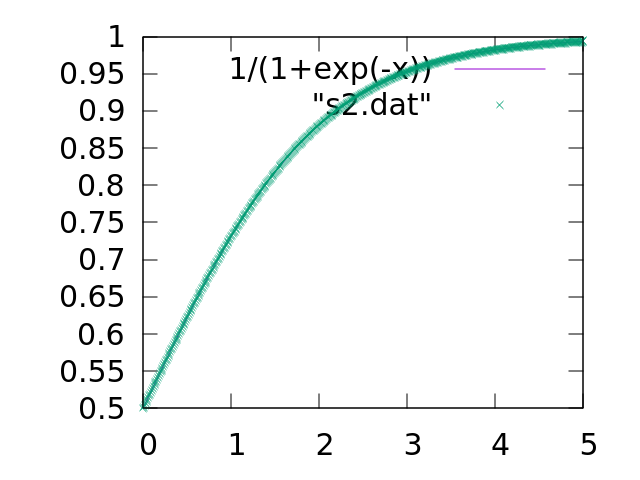
\includegraphics[scale=1.00]{s2solu.png}
		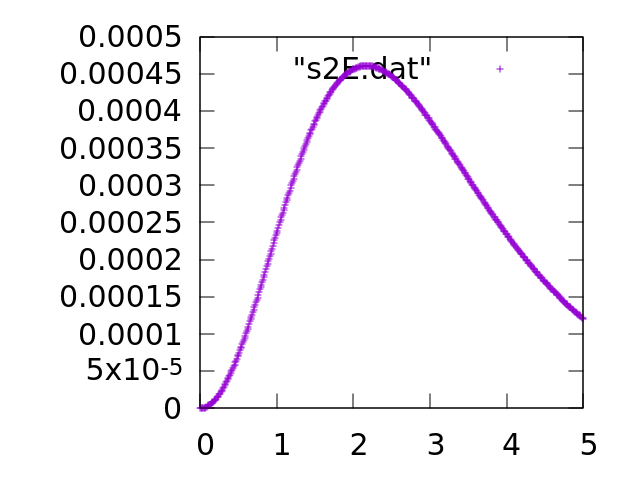
\includegraphics[scale=1.00]{s2err.png}\\
		\item Approximation of $x'(t) = \cos(x^3(t)) - \cos(x^2(t) -3t), x(0) = 1 $.\\
		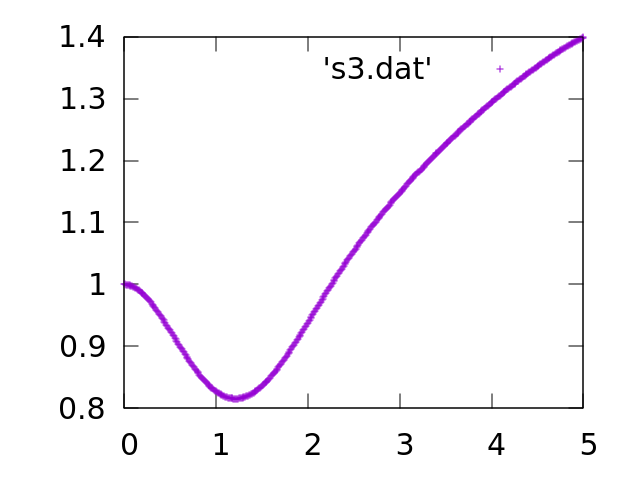
\includegraphics[scale=1]{s3solu.png}
		\item ~\\
		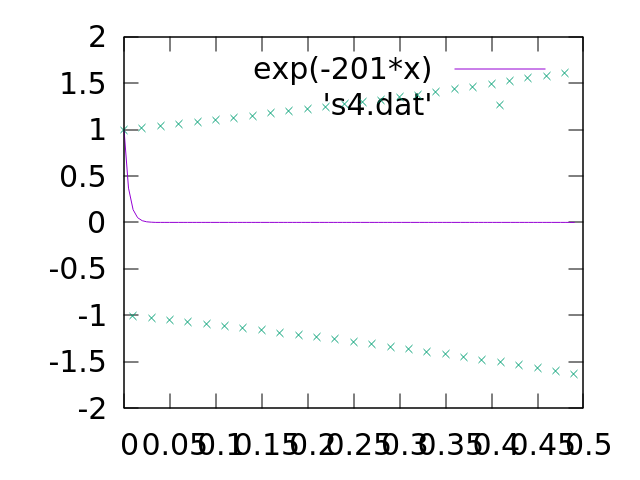
\includegraphics[scale=1]{s4badSolu.png}
		\item ~\\		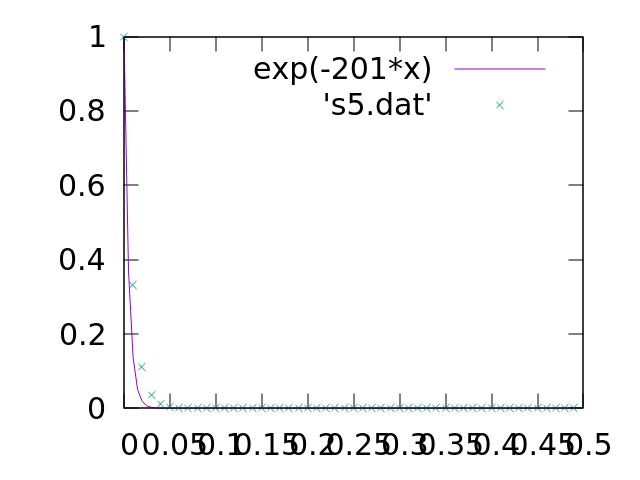
\includegraphics[scale=1]{s5solu.png}
		\item The order of the greatest error is $10^{-6}$.  Compared to the standard Euler method, the error is 3 orders of magnitude less.\\
		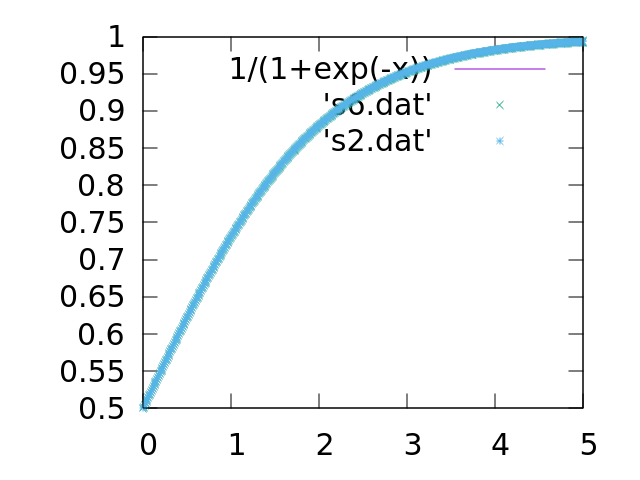
\includegraphics[scale=1]{s6solu.png}
		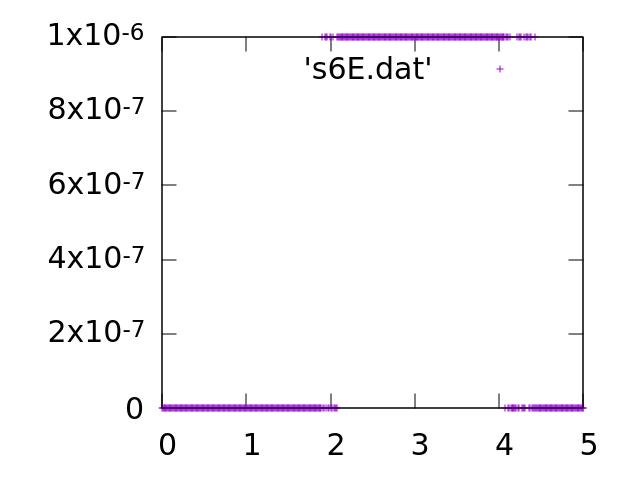
\includegraphics[scale=1]{s6err.png}
	\end{enumerate}
\end{document}